\section{Relative Luminosity Determination}

Bunch-by-bunch beam luminosities are measured using the BBCs and ZDCs and
recorded via the Scaler Boards. The detectors are described in
Sections~\ref{sec:bbc}, \ref{sec:zdc}, and \ref{sec:scalers}. The BBC
measurements are more precise and are employed in the calculation of \(A_{LL}\);
the ZDCs provide a cross-check essential for evaluating systematic
uncertainties.

Various bits of information related to BBC coincidences were encoded on several
Scaler Boards during the 2005 and 2006 RHIC runs. A detailed QA and comparison
of the different boards led to the conclusion that the fine-grained timing
information on boards 5 and 6 should be used to calculate the relative
luminosities. These boards allocated enough bits to track the BBC coincidences
in 16 buckets in \(\Delta T\), the time difference between a hit in the East BBC
and the West BBC. Board 5 was configured to integrate throughout each \(\sim\)
40 minute long STAR run, while board 6 took samples every 250 seconds to allow a
determination of the relative luminosity stability throughout a run.

When possible, the relative luminosities for a run are calculated using the
measurements from board 5. A small number of otherwise-acceptable 2006 runs do
not have reliable scaler information from board 5; in these cases the analysis
relies on the data from board 6. The bunch crossing spin assignments are
obtained using the procedure described in Section \ref{sec:spindb}. The
coincidence count for each bunch crossing is restricted to a set of time buckets
chosen to approximate a 60~cm cut on the $z$ position of the vertex; in the 2005
analysis buckets 7, 8, and 9 are selected, while the 2006 analysis adds bucket 6
into the sum. The relative luminosity \(R\) for a run is then simply the sum of
BBC coincidences in the selected set of time buckets for the bunch crossings
with \(++\) or \(--\) spin assignments divided by the same quantity for bunch
crossings determined to be in a \(+-\) or \(-+\) spin configuration.

% remove runs less than 60 seconds long

% remove runs where the time-integrated BBC coincidence in bit16 < 10k

% remove runs with large number of counts in abort gaps, maybe

% require data from 5/6/11/12, as well as multiple scaler files for the sampling boards

% require that the relative luminosity is fairly stable throughout a fill -- |max(R3) - min(R3)| < 0.0001

% use bit16 on boards 11 and 12, but per-timebin info on boards 5 and 6 (guessing that 11 and 12 don't have timebin info)

% some discrepancies between STAR run stop time and scaler timestamp.  STAR started "getting ahead" of scaler system.  Was anything done about this?  Not clear.  I don't think so

% what was the difference between release 1 and release 2?

\begin{figure}
  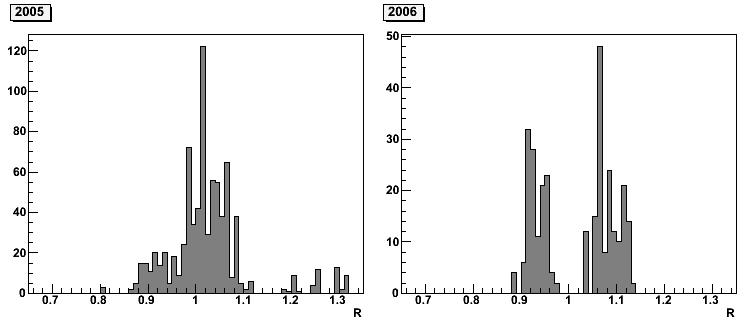
\includegraphics[width=1.0\textwidth]{figures/relative_luminosities}
  \caption{Distributions of per-run values for $R = \frac{\mathcal{L}_{++}}{\mathcal{L}_{+-}}$}
\end{figure}

The statistical uncertainties on $A_{LL}$ assume perfect knowledge of the
relative luminosity of the different spin states. That simplification is
addressed via the systematic uncertainty evaluation described below.

\subsection{Uncertainty Evaluation Using the ZDCs}

% \textit{Note: \href{http://mare.tamu.edu/star/2005n06Jets/2005relLumSys_mar29_2008/}{analysis by Murad Sarsour}}

We can quantify the precision with which we understand the relative luminosities
obtained from the BBCs by using an independent luminosity monitor, the ZDCs. In
the absence of non-statistical fluctuations, the uncertainty on R will be
dominated by the statistics in the ZDCs, which count at a much lower rate than
the BBCs during proton-proton running.

A couple of problems in the ZDC data need to be corrected before a comparison
to the BBCs can be trusted. The first problem is due to the ``killer bit''
algorithm, which suppressed signals in the ZDCs for 10 bunch crossings after
an initial signal. The algorithm is used in heavy ion running to prevent
ringing in the calorimeters from generating false signals, but in pp running
it biases the ZDC counts. Bunch crossings immediately following abort gaps
(where the killer bit is more likely to be off) end up with more ZDC counts
than crossings in the middle of a filled set of bunches. As a result, the
ratio of relative luminosities obtained from the ZDC and BBC will not be flat,
see Figure \ref{fig:zdctobbc6170012zoom}.

\begin{figure}
  \includegraphics[width=1.0\textwidth]{figures/ZDCtoBBC_r7138003}
  \caption{Ratio of uncorrected ZDC and BBC coincidences versus bunch crossing.  The ratio is larger in bunch crossings immediately following abort gaps.}
  \label{fig:zdctobbc6170012zoom}
\end{figure}

The procedure developed to correct for this effect requires scaling the counts
for a given bunch crossing by a factor that takes into account the frequency
with which the previous ten bunch crossings had a signal. For the ZDC singles
rates, the formula for the corrected counts $n_{j}$ in a given bunch crossing
$j$ is
%
\begin{equation}
  n_{j}^{corrected} = n_{j} * \frac{N_{cycles}}{N_{cycles} - \sum_{i=1}^{10}n_{j-i}}
\end{equation}
%
where $N_{cycles}$ is the number of times the beam cycled through STAR in the
run. Figure \ref{fig:zdc-singles-ratio} shows the effect of applying the
correction for a sample run.

\begin{figure}
  \subfloat{
    \includegraphics[width=0.5\textwidth]{figures/ZDCtoBBC_r7133049ER}
  }
  \subfloat{
    \includegraphics[width=0.5\textwidth]{figures/ZDCtoBBC_r7133049WR}
  }
  \caption{Change in the ZDC singles rates after applying the killer bit correction.}
  \label{fig:zdc-singles-ratio}
\end{figure}

The formula to correct the ZDC coincidence counts is complicated by the need to
track the killer bits for the two detectors simultaneously. The formula for the
corrected coincidence counts \(c_{j}^{corrected}\) in a bunch crossing given raw
singles counts \(e_{j}\) (ZCDE) and \(w_{j}\) (ZDCW) and coincidence counts
\(c_{j}\) is
%
\begin{align}
  &\alpha_{j} = N_{cycles} - \sum_{i=1}^{10}c_{j-i} \notag\\
  &\beta_{j} = E_{j-10} + W_{j-10} + E_{j-9}*\left(1 - \frac{W_{j-10}}{\alpha_{j} - E_{j-10}}\right) + W_{j-9}*\left(1 - \frac{E_{j-10}}{\alpha_{j} - W_{j-10}}\right) + ...\notag\\
  &c_{j}^{corrected} = c_{j} * \frac{N_{cycles}}{\alpha_{j} - \beta_{j}} 
\end{align}
%
where \(E(W)_{j-i} \equiv e(w)_{j-i} - c_{j-i}\) is the ZDCE(W) singles count
minus the coincidence count for the j-ith bunch crossing. The effect of the
killer bit correction on the coincidence distributions is shown in Figure
\ref{fig:coinRat6143016}.

\begin{figure}
  \begin{center}
    \includegraphics[width=0.6\textwidth]{figures/ZDCtoBBC_r7133049coin}
  \end{center}
  \caption{Change in the ZDC coincidence rates after applying the killer bit
  correction.}
  \label{fig:coinRat6143016}
\end{figure}

\begin{figure}
  \begin{center}
    \includegraphics[width=0.8\textwidth]{figures/c7308}
  \end{center}
  \caption{Example of a coherent spin pattern and even-odd ZDC rate
  oscillation. In this case, the ZDC rate is always higher when the spin of
  the blue beam is down.}
  \label{fig:c7308}
\end{figure}

% More Details on even-odd effect
% http://cyclotron.tamu.edu/star/2006Jets/jul31_2007/
% http://cyclotron.tamu.edu/star/2006Jets/aug2_2007/ - figure 4 on this page plots the asymmetry between the ZDC/BBC ratio for even bxings and the ZDC/BBC ratio for odd bxings.  The asymmetry can be positive or negative even within a spin pattern, basically no correlation.  But at the bottom of the page, Murad clearly shows that the even/odd asymmetry arises from the ZDCs, not the BBCs, when he plots a particular jet asymmetry using R_ZDC and then R_BBC, and compares the sign of that asymmetry to the sign of the asymmetry in Figure 4.

% the cut on |F*(S-1)| < 0.002 is strictly a 2005 thing, in 2006 the ZDC coincidences are actually renormalized! Uber-sketchy if you ask me.

The second problem in need of correction has come to be known as the
``even-odd'' effect.  The ZDC coincidence rates are often
different for even-numbered and odd-numbered bunch crossings, due to
oscillations in the electronics pedestals in specific ADC channels of the CDB
boards used to read out the ZDCs. This oscillation can introduce a false
asymmetry if it aligns coherently with a particular spin pattern. For instance,
in Figure \ref{fig:c7308} the ZDC coincidence rates are always higher when the
spin of the blue beam is down.  To quantify the bias this introduces on $A_{LL}$, we can
define the fractional overlap between the even-odd ZDC oscillation and relevant
portion of the spin pattern for $A_{LL}$ using a 120 element vector $|EO\rangle
= |+1,-1,+1,-1,...\rangle$ and another 120 element vector $|LL\rangle$ whose
elements are 1 if the bunch crossing is UU or DD, -1 if UD or DU, and 0
otherwise. The inner product of these vectors measures the susceptibility of
$A_{LL}$ for that spin pattern to any even-odd oscillation.

% \begin{figure}
%   \includegraphics[width=1.0\textwidth]{figures/fevfod}
%   \caption{Magnitude of even-odd rate asymmetry versus time in the 2005 RHIC run.}
%   \label{fig:fevfod}
% \end{figure}

It turns out that $A_{LL}$ is less biased by the even-odd rate oscillation in
the ZDC than, say, the blue beam single-spin asymmetry. Figure \ref{fig:cll}
plots the fill-by-fill change in $A_{LL}$ if the ZDC is used for relative
luminosities instead of the BBC against the the product of the fractional
overlap $F \equiv \langle EO | LL \rangle$ and the magnitude of the even-odd
oscillation $S-1$. Placing a cut on $|F*(S-1)| < 0.002$ is well-motivated. For
fills without reliable ZDC information, we use Figure \ref{fig:fevfod} to
assume a conservative $|S-1| = 0.03$.

\begin{figure}
  \begin{center}
  \includegraphics[]{figures/cll}
  \end{center}
  \caption{Change in $A_{LL}$ versus the product of the even-odd rate oscillation amplitude and the fractional overlap $\langle EO | LL \rangle$.  Deviations from 0 on the x-axis indicate fills where $A_{LL}$ is biased by the even-odd effect.}
  \label{fig:cll}
\end{figure}

After correcting for the killer bits and rejecting the fills that fail the
even-odd oscillation cut the ZDC coincidences counts for even and odd bunch
crossings are separately normalized using the following normalization factors:
%
\begin{equation}
  f_{even} = \frac{\langle ZDC/BBC \rangle}{\langle ZDC_{even}/BBC_{even} \rangle}, ~~~~
  f_{odd} = \frac{\langle ZDC/BBC \rangle}{\langle ZDC_{odd}/BBC_{odd} \rangle};
\end{equation}
%
that is, the ZDC coincidence counts for even(odd)-numbered bunch crossings in a
run are rescaled by the mean ZDC/BBC ratio for the run divided by the mean
ZDC/BBC ratio for even(odd)-numbered bunch crossings in the run. Finally, the
uncertainty on $A_{LL}$ due to the uncertainty in the relative luminosities is
calculated as the change in \(A_{LL}\) when the relative luminosities are
supplied by the normalized ZDCs instead of the BBCs, and is equal to
$9.4\times10^{-4}$.

% \subsection{Beam Background Bias}
% 
% % \textit{Note: \href{http://www.star.bnl.gov/protected/spin/kowalik/2005/r-lumi/bkg_sys.html}{analysis by Kasia Kowalik}}
% 
% The relative luminosities obtained from the BBCs might also be biased by false
% signals generated by beam-gas background. We can try to quantify this by
% studying the coincidence rate in crossings where one of the two beams has an
% unfilled bunch (``abort gaps''). The beam-gas background is assumed to be
% crossing- and spin-independent, but it can be different in each beam. It follows
% that the per-crossing coincidence rate due to beam-gas in each beam is just the
% average number of BBC coincidences found in the abort gaps for that beam. In
% Figure \ref{fig:bkg-yellow-blue}, the x-axis is the background rate divided by
% the total rate, defined as the average number of coincidences per bunch crossing
% with a spin state of \(++\), \(+-\), \(-+\), or \(--\). The two histograms are
% incremented for each STAR run. We see that the background rate in the BBCs due
% to beam-gas is typically less than 0.1\% of the total rate.
% 
% \begin{figure}
%   \includegraphics[width=1.0\textwidth]{figures/bkg-yellow-blue}
%   \caption{Fraction of the total coincidence rate attributed to beam gas in
%   each beam. The histograms are incremented once for each STAR run.}
%   \label{fig:bkg-yellow-blue}
% \end{figure}
% 
% Given run-dependent background fractions for both beams, it's possible to
% calculate background-subtracted relative luminosities. Figure
% \ref{fig:r-lumi-sys-bkg} shows the difference between the raw relative
% luminosity and the background-subtracted version. The background-corrected
% relative luminosities yield an $A_{LL}$ that differs from the original by
% $3.0\times10^{-4}$, so we use that as the uncertainty for this source of
% systematic error.
% 
% \begin{figure}
%   \begin{center}
%     \includegraphics[width=0.6\textwidth]{figures/r-lumi-sys-bkg}
%   \end{center}
%   \caption{Change in the relative luminosities after correcting for beam-gas
%   background.}
%   \label{fig:r-lumi-sys-bkg}
% \end{figure}
